%****************************************************************
% Chapter X
%****************************************************************
\label{chapter-technology}
\chapter{Technology}

In this chapter, details of the related technologies are presented. They are Android smartphone, a low-cost way to experience immersive virtual reality environment; OpenGL ES in Android; KML for geographic visualization; Golang RESTful web server for managing data in the back-end.

%****************************************************************
\section{Virtual Reality Device}

There are following reasons for using Android smartphone as the virtual reality device. The intention is to identify immersive virtual reality device that not only low-cost but also a standard, customer-friendly device. That is the smartphone, and it had an incredibly fast growth trend in the last few years and a good promising market prospect \ref{fig:smartphone-shipments-forecast}. After all, it contains all the necessary sensors and positioning systems to measure motion and accurately track device movements - Six degrees of freedom (DOF) - position coordinates (x, y and z offsets) and orientation (yaw, pitch and roll angles). Additionally, 15\$ Google Cardboard kit turns Android or iOS smartphone to immersive virtual reality device. According to International Data Corporation (IDC), Android dominated the smartphone market with a share of 87.6\% in the worldwide \ref{fig:smartphone-os-market-share}. Moreover, there is an existing Google VR SDK \cite{google.vr-sdk.2016} for Android supports.

\begin{figure}[H]
\caption[Global Smartphone Shipments Forecase]{Global Smartphone Shipments Forecase \cite{tony.global-smartphone-market.2015}}
\label{fig:smartphone-shipments-forecast}
\centering
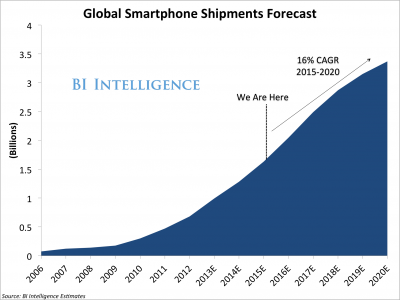
\includegraphics[]{Figures/smartphone-shipments-forecast.png}
\decoRule
\end{figure}

\begin{figure}[H]
\caption[Smartphone OS Market Share]{Smartphone OS Market Share \cite{idc.smartphone-os-market-share.2016}}
\label{fig:smartphone-os-market-share}
\centering
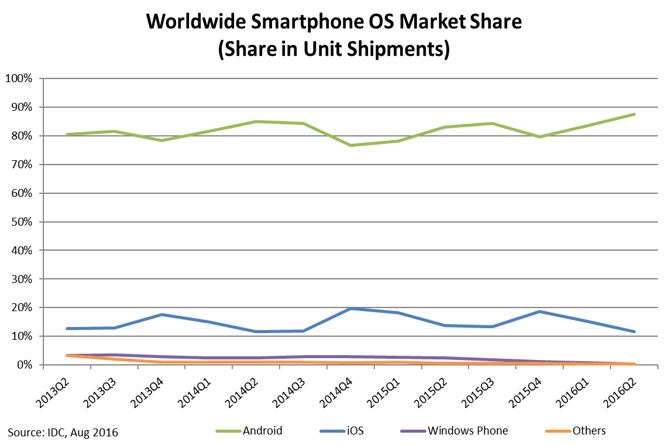
\includegraphics[width=\linewidth]{Figures/smartphone-os-market-share.png}
\decoRule
\end{figure}

%****************************************************************
\section{OpenGL ES}

Android includes support for high-performance 2D and 3D graphics with the Open Graphics Library, specifically, the OpenGL ES API \cite{google.opengles.2016}. OpenGL ES is a branch of the OpenGL specification intended for embedded devices. The Google VR SDK requires the device has a minimum OpenGL ES 2.0 support. Table \ref{tab:opengles-spec-android} shows a version list of OpenGL ES API that Android supported.

\begin{table}[H]
\caption{OpenGL ES API specification supported by Android}
\label{tab:opengles-spec-android}
\centering
\begin{tabular}{l l l}
\toprule
\tabhead{OpenGL ES Version} & \tabhead{Android Version}\\
\midrule
OpenGL ES 1.0 & Android 1.0 and higher\\
OpenGL ES 1.1 & Android 1.0 and higher\\
OpenGL ES 2.0 & Android 2.2 (API level 8) and higher\\
OpenGL ES 3.0 & Android 4.3 (API level 18) and higher\\
OpenGL ES 3.1 & Android 5.0 (API level 21) and higher\\
\bottomrule
\end{tabular}
\end{table}

%****************************************************************
\section{Geographic Visualization Markup Language}

We were looking for a simple markup language that we can publish and consume data  in interoperable formats without the need for technical assistance. In the \ref{section:background}, we introduced KML (it can be combined with other supporting files such as imagery in a zip archive, producing a KMZ file), which is the markup language we are using in the project. It is not only because it can simply satisfy our application purpose, more importantly, it is supported by many virtual globes and other GIS systems and is therefore already becoming a de facto standard \cite{blower.sharing-visualizing.2007}. Moreover, the annotations of KML features are not designed as machine-readable XML, but a human readable plain text or simple HTML. Moreover, real-time data are important in the environmental sciences. The Networklink facility in KML allows all or part of the dataset to be automatically refreshed by the URL, to ensure the user always sees the latest information.

From an environmental science point of view, KML is a somewhat limited language. It can only describe simple geometric shapes on the globe (points, lines, and polygons) and is not extensible. It is, in many respects, analogous to Geography Markup Language (GML) 3.0+ is much more sophisticated and allows the rich description of geospatial features such as weather fronts and radiosonde profiles. For the above reasons, KML is currently not suitable as a fully-featured, general-purpose environmental data exchange format. Nonetheless, it earns the acceptance from an increasing number of scientists. It is important to be aware of that virtual geographic data visualization (and KML) do not attempt to replace more sophisticated systems. 

Figure \ref{fig:kml-schema} shows the KML schema. From the point of view of usability, KML spans a gap between very simple (e.g. GeoRSS) and more complex (GML) formats, that makes it easy for non-technical scientists to share and visualize simple geospatial information which can then be manipulated in other applications if required. 

\begin{figure}[H]
\caption[KML schema]{KML schema \cite{google.kml.2016}}
\label{fig:kml-schema}
\centering
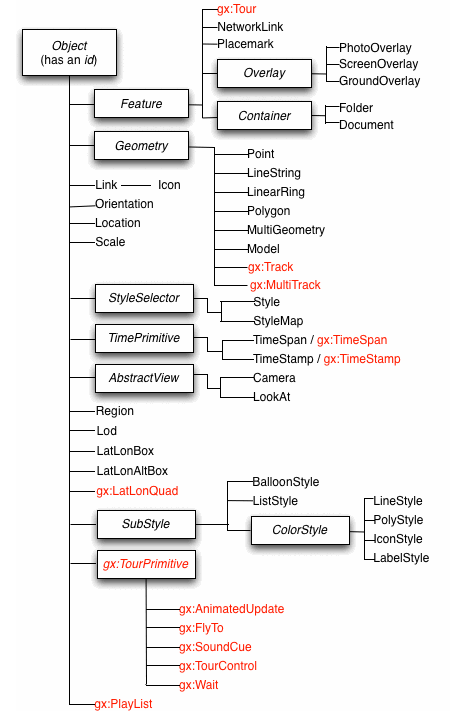
\includegraphics[]{Figures/kml-schema.png}
\decoRule
\end{figure}

%****************************************************************
\section{Web Server}
\label{section:network}

The key strengths of virtual reality applications are not only easy-to-use, and intuitive nature, but also the ability to incorporate new data very easily. Therefore, real-time data are very important in the environmental sciences \cite{blower.sharing-visualizing.2007}. To do that, a web server is needed. In this project, we implemented a RESTful web server to support communication with the client, along with a  file server to synchronize data. In the client side.

Go (often referred to as golang \cite{google.golang.2016}) is an open source programming language, and it is compiled, concurrent, garbage-collected, statically typed language developed at Google in late 2007. It was conceived as an answer to some of the problems we were seeing developing software infrastructure \cite{google.talk-golang.2012}. Also, it growing fast that each month the contributors outside Google is already more than contributors inside the Go team.

We are using Go to build the server, it is well suited for developing RESTful API’s. The net/http standard library provides key methods for interacting via the HTTP protocol. On the other hand, since our client is Android phone, we introduced Volley for transmitting network data (Volley is an open sourced HTTP library that makes networking for Android apps easier and most importantly, faster \cite{google.volley.2016}), and jsoup (Java HTML Parser \cite{joup.2016}) for analyzing HTML format response.

%****************************************************************
